\chapter{Polarizace}
Polarizace je vlastnost všech harmonických vlnění s možností kmitání ve více jak jednom směru, kterým je například i světlo. V tomto případě popisuje orientaci elektrického pole v prostoru, kde se vlna šíří. V této kapitole se bude zabýat šířením nevodivým homogením izotropním prostředím. V takovém případě je EM vlna příčná a navíc platí mezi elektrickou intenzitou $\vec{E}$ a magnetickou indukcí $\vec{B}$ vztah
\begin{eqnarray}
\vec{B}=\frac{1}{v}(\vec{s}\times\vec{E}),
\end{eqnarray}
kde $\vec{s}$ je jednotkový vektor ve směru šíření. Díky tomuto vztahu nám tedy popis elektrického pole dá úplnou informaci o celém EM poli. Elektrické pole bylo zvoleno, především kvůli jeho výrazně větším silovým účinkům.
K popisu vektoru elektrické intenzity budeme používat komplexní symboliku. Nejjednoduší případ je rovinná vlna, jejíž předpis můžeme obecně zapsat ve tvaru
\begin{eqnarray}
\vec{E}=Re(\vec{E_0}exp(-i(\omega(t-\frac{\vec{r}\vec{s}}{v})+\varphi))),
\label{rovinna vlna}
\end{eqnarray}
kde $\vec{E_0}$ značí amplitudu vlny, $i\omega$ úhlovou frekvenci, $\vec{s}$ jednotkový vektor ve směru šíření a $\varphi$ fázový posun vlny.

Dále si můžeme zvolit soustavu souřadnou tak, aby $\vec{s}$ mířil ve směru osy z. Díky tomu víme, že z-tová složka elektrické intenzity bude nulová a rovnici (\ref{rovinna vlna}) můžeme  přepsat do tvaru
\begin{eqnarray}
\vec{E}(z,t)=E_x\vec{x}+E_y\vec{y} \\
E_x=a_x\cos(\tau+\varphi_x) \label{Ex}\\
E_y=a_y\cos(\tau+\varphi_y) \label{Ey}\\
\tau=\omega(t-\frac{z}{v}))
\end{eqnarray}
Úpravami rovnic (\ref{Ex}) a (\ref{Ey}) a jejich následným sečtením můžeme docílit vztahu
\begin{eqnarray}
\left(\frac{E_x}{a_x}\right)^2+\left(\frac{E_y}{a_y}\right)-2\frac{E_xE_y}{a_xa_y}\cos(\varphi_y-\varphi_x)=\sin^2(\varphi_y-\varphi_y),
\end{eqnarray}
jenž je rovnicí elispy. Z toho vyplývá, že úplně polarizované světlo má obecně eliptickou polarizace. Tato elispa může být definována různě, proto na obrázku (\ref{polarizacni elipsa}) naleznete vyznačené nejčastěji užívané parametry. Důležité je, že pro úplný popis potřebujeme čtyři parametry. Pokud nás nezajímá počátek času, vystačíme si jen se třemi. Dále používané parametry po popis polarizace tedy budou
\begin{enumerate}
\item a,b\dots hlavní a vedlejší poloosa
\item $\psi\in[-\pi/2,\pi/2]$\dots azimut
\item $\chi\in[-\pi/2,\pi/2]$\dots úhel elipticity
\end{enumerate}
Úhle elipticity může nabývat i záporných hodnot, protože znaménko v sobě informaci o směru otáření vektoru elektrické intenzity. V naší konvenci máme pro pravotočivé světlo kladné hodnoty a pro levotočivé záporné. Nula odpovídá lineárně polarizovanému světu, kdy vektor elektrické intenzity kmitá pouze v rovině. Tato rovina se nazývá rovinnou polarizace. Mezi další význačné polarizace patří kruhově polarizované světlo, kdy $a_x=a_y$ a fázový posun $\varphi=\varphi_y-\varphi_x$ je $\pi/2$ pro pravotočivé a $-\pi/2$ pro levotočivé světlo.

Tento popis polarizace světla je sice úplný, ale pro praktické účely zcela nevhodný. Z toho důvodu vzniklo mnoho formalizmů pro zjednodušení popisu svěla a jeho interakci s optickými elementy. Pro náš případ je nejběžněji používaný maticový popis za pomoci takzvaných Jonesových vektorů.

\begin{figure}
\begin{center}
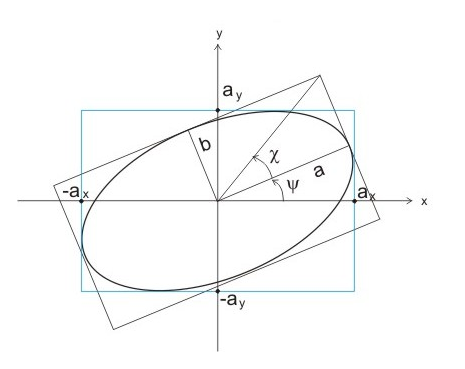
\includegraphics[width=5in]{img/polarelip.eps}
\caption{Polarizační elispa}
\label{polarizacni elipsa}
\end{center}
\end{figure}

\section{Jonesovy vektory a matice}
Tento formalizmus slouží pouze pro popis zcela polarizovaného světla, což by se mohlo zdát velmi omezující, ale pro potřeby této práce s ním bohatě vystačíme. Jak bylo zmíněno výše, rovinnou elektromagneticou vlnu můžeme v komplexní symbolice zapsat
\begin{eqnarray}
\vec{E}(z,t)=E_x\vec{x}+E_y\vec{y} \\
E_x=a_xe^{-i(\omega t-kz+\varphi_x)}=A_xe^{-i(\omega t-kz)}\\
E_y=a_ye^{-i(\omega t-kz+\varphi_y)}=A_ye^{-i(\omega t-kz)},
\end{eqnarray}
kde členy $A_i$ nazveme komplexní obálkou. Díky nim můžeme definovat vektor
\begin{eqnarray}
\vec{J}=\begin{bmatrix} A_x \\ A_y \end{bmatrix},
\end{eqnarray}
který nazveme Jonesovým vektorem polarizace. Tento vektor nese plnou informaci o polarizačním stavu světla. Jako příklad uvedu pár významných polarizací popsaných za pomoci tohoto formalizmu.
\begin{enumerate}
\item lineárně polarizované v ose x $\begin{bmatrix} 1 \\ 0 \end{bmatrix} \dots báze lineárních polarizací$
\item pravotočivě kruhově polarizované světlo $\begin{bmatrix} 1 \\ -i \end{bmatrix} \dots báze kruhových  polarizací$
\end{enumerate}
Jakoukoliv polarizaci niní můžeme popsat ve tvaru
\begin{eqnarray}
\vec{J}=\alpha_1\vec{J_1}+\alpha_2\vec{J_2}
\end{eqnarray}
kde dvojici vektorů $\vec{J_i}$ volíme ortogonální vzhledem skalárnímu součinu $(\vec{J_1},\vec{J_2})=J_{1x}J_{2x}^*+J_{1y}A_{2y}^*$. Nejběžněji používané  baze jsou
\begin{enumerate}
\item $\vec{J_x} = \begin{bmatrix} 1 \\ 0 \end{bmatrix}$, $\vec{J_y} = \begin{bmatrix} 0 \\ 1 \end{bmatrix}$
\item $\vec{J_-} =  \frac{1}{\sqrt{2}} \begin{bmatrix} 1 \\ -i \end{bmatrix}$, $\vec{J_+} = \frac{1}{\sqrt{2}} \begin{bmatrix} 1 \\ +i \end{bmatrix}$
\end{enumerate}
Když máme dobře popsáno světlo, můžeme se přesunout k jeho interakci s optickým prvkem (například čočkou či polarizátorem). Ten můžeme popsat za pomci matice 2x2. Vektor popisující světlo po interakci s prvkem popsaným maticí $\mathbb{T}$ pak získáme z jednoduché rovnice
\begin{eqnarray}
\vec{J_2}=\mathbb{T}\vec{J_1}
\end{eqnarray}
analogicky bychom mohli postupovat pro soustavu $n$ optických prvků, pro kterou bychom získali
\begin{eqnarray}
\vec{J_n}=\mathbb{T}_n...\mathbb{T}_1\vec{J_1}
\end{eqnarray}
Nyní si uvedeme několik matic popisujících optické prvky, které budou dále použity. Nejprve v bázi lineárních polarizací.
\begin{enumerate}
\item polarizátor natočený o úhel $\alpha$ od osy x $\begin{bmatrix} \cos^2\alpha & \sin\alpha\cos\alpha \\ \sin\alpha\cos\alpha & \sin^2\alpha \end{bmatrix}$
\item fázová destička s fázovým posunem o úhel $\delta$ a rychlou osou ve směru x $\begin{bmatrix} e^{i\frac{\delta}{2}} & 0 \\ 0 & e^{-i\frac{\delta}{2}} \end{bmatrix}$
\item polarizační rotátor stáčející rovinu polarizace o úhle $\vartheta$ $\begin{bmatrix} \cos\vartheta & -\sin\vartheta \\ \sin\vartheta & \cos\vartheta \end{bmatrix}$
\end{enumerate}
a následně v bázi kruhových polarizací
\begin{enumerate}
\item polarizátor natočený o úhel $\alpha$ od osy x  $\frac{1}{2}\begin{bmatrix} 1 & e^{2i\alpha} \\ e^{-2i\alpha} & 1 \end{bmatrix}$
\item fázová destička s fázovým posunem o úhle $\delta$ a rychlou osou ve směru x  $\begin{bmatrix} \cos\frac{\delta}{2} & i\sin\frac{\delta}{2} \\ i\sin\frac{\delta}{2} & \cos\frac{\delta}{2} \end{bmatrix}$
\item polarizační rotátor stáčející rovinu polarizace o úhel $\vartheta$ $\frac{1}{2}\begin{bmatrix} e^{i\vartheta} & 0 \\ 0 & e^{-i\vartheta} \end{bmatrix}$
\end{enumerate}
Velmi užitečný je vztah vztah pro transformaci matice elementu, kterou zíkáme matici odpovídající prvku otočenému o úhel $\vartheta$
\begin{eqnarray}
T'=R(\vartheta)TR(-\vartheta), \\
R(\vartheta) = \begin{bmatrix} \cos\vartheta & \sin\vartheta \\ -\sin\vartheta & \cos\vartheta \end{bmatrix}.
\end{eqnarray}
Jonesovy matice můžeme také transformovat do bází odpovídající zvojené bázové dvojici Jonesových vektorů. Zde platí vztah podobný jako vztah uvedený výše (Lze na něj nahlížet jako změnu báze na vektory pootočené o úhel $\theta$)
\begin{eqnarray}
T'=F^{-1}TF
\end{eqnarray}
kde $F$ značí matice přechodu z nečárkované baze do baze čárkované. Podrobnosti se dají najít v leckteré učebnici lineární algebry, jako je třeba [\cite{Smid}].

\section{Interakce se vzorkem}
V předchozích odstavcích bylo vysvětleno, jak můžeme popsat světlo po průchodu optickou soustavou. Jako poslední nám tedy chybí řešení porblému, kdy se v soustavě vyskytuje neznámý prvek. Tento element můžeme opět popsat Jonesovou maticí, která má obecně čtyři komplexní prvky. Ve skutečnosti jsou tyto matice dvě, protože vzorek se chová jinak pro odraz a jinak pro průchod. Tyto matice si nejprve označíme
\begin{eqnarray}
S^{sp}_R = \begin{bmatrix} r_{ss} & r_{sp} \\ r_{ps} & r_{ss} \end{bmatrix} \\
S^{sp}_T = \begin{bmatrix} t_{ss} & t_{sp} \\ t_{ps} & t_{ss} \end{bmatrix} 
\end{eqnarray}
kde $s$ respektive $p$ značí, že používáme za bázi s-polarizované respektive p-polarizované světlo, R  reflexi a T trasmisi. Směr $p$ a $s$ polarizace je dán rovinou dopadu, přičemž $p$ je na ni kolmá a $s$ rovnoběžná. Pro isotropní materiál bez přítomnost magnetického pole je tato matice diagonální, tedy nedochází k žádné interakci mezi $s$ a $p$ vlnami. Po zapnutí magnetického pole jsou nediagonální elemnety obecně nenulové. V případě, že máme radiálně symetrický prvek (a to např včetně mag. pole) platí užitečný vztah
\begin{eqnarray}
R(\alpha)S^{sp}_RR(\alpha)=S^{sp}_R \\
R(-\alpha)S^{sp}_TR(\alpha)=S^{sp}_T
\end{eqnarray}
kde $R(\alpha)$ značí matici rotace o úhel $\alpha$.
Z maticových rovnic zíksáme celou řadu vztahů pro maticové elementy
\begin{eqnarray}
r_{ps}&=&r_{sp} \\
t_{ps}&=&-t_{sp} \\
r_{pp}&=&-r_{ss} \\
t_{pp}&=&t_{ss} \\
r_{sp}(-\vec{M})&=&-r_{sp}(\vec{M}) \\
t_{sp}(-\vec{M})&=&-t_{sp}(\vec{M}) \\
r_{ss}(-\vec{M})&=&r_{ss}(\vec{M}) \\
t_{ss}(-\vec{M})&=&r_{ss}(\vec{M}) \\
t_{ss}(-\vec{M})&=&t_{ss}(\vec{M})
\end{eqnarray}
kde $\vec{M}$ značí vektor magnetizace.
V praxi se nepoužívají k popisu maticové elementy, ale veličiny Kerrovy (Faradayovy) rotace ($\theta$)  a elipticity ($\epsilon$), které jsou definovány
\begin{eqnarray}
-\frac{r_{ps}}{r_{ss}}=\Theta_{Ks} \approx \theta_{Ks} -i\epsilon_{Ks} \\
\frac{t_{ps}}{t_{ss}}=\Theta_{Fs} \approx \theta_{Fs}-i\epsilon_{Fs} \\
\frac{r_{sp}}{t_{pp}} = \Theta_{Kp} \approx \theta_{Kp} -i\epsilon_{Kp}\\
-\frac{t{sp}}{t_{pp}} = \Theta_{Fp} \approx \theta_{Fp}-i\epsilon_{Fp}
\end{eqnarray}
Pro kolmý dopad dále platí, že $\Theta_{Ks}=\Theta_{Kp}=\theta_K$. To samé platí i pro koeficienty transmise. Po normalizaci pak získáme matice popisující vzorek ve tvaru
\begin{eqnarray}
S_R^{sp}&=&\begin{bmatrix}1&-\Theta_K \\ -\Theta_K & -1 \end{bmatrix} \\
S_T^{sp}&=&\begin{bmatrix}1&-\Theta_F \\ \Theta_F& 1 \end{bmatrix}
\end{eqnarray}
Pokud tyto matice transformujeme do báze kruhových polarizací, získáme
\begin{eqnarray}
S_R^{LR}&=&\begin{bmatrix}0 & r_{ss}\\ r_{ss}-ir_{ps}&0\end{bmatrix} \\
S_T^{LR}&=&\begin{bmatrix}t_{ss} & 0 \\ 0& t_{ss}-it_{ps}\end{bmatrix}
\end{eqnarray}
